\chapter{Test Bench}\label{ch:test_bench}
In the first stages of the work on the dependable communication system, there was a need for functional testing of encoder and decoder systems designed by Petr Pfeifer. The main purpose was to find the limits of the designs. The later step was to build up a communication path and propose a testing scenario for the system as a whole. Both tasks required a development of a test platform to feed the designs with input data and gather the responses.

The standard approach, in building a test bench consists in creating a non-synthesizeable HDL description, generating the test patterns and simulating the design, using the development environment. The simulation is very time consuming and not suitable for larger test sets. The creation of synthesizeable test bench is legitimate when one wants to create a universal test environment for many different designs with the ability to provide external test patterns and test the design in the "real" hardware. The test results will still be just approximations, due to logic mapping and routing in the FPGA and very sensitive to changes in synthesis and placement parameters. There is but no other more precise tool to test ones design before the manufacturing process.

The main idea behind the test bench development was to make it configurable and adaptable. The test bench has been developed parallel to the system and therefore has been redesigned to suit the current needs. It became clear that it has to be able to conduct various tests on any design with adjustable frequencies and not be bound to any design or interface in particular. The general idea of testing a design has been shown in \autoref{fig:test}.

The test bench is responsible for applying the test vectors to the inputs of the UUT and recording the responses. The generation of test patterns, systematic or random, and response evaluation must be repeated for every design tested, therefore this is the responsibility of the test designer. The easiest interface from the users perspective is a PC application acting as the GUI to the test bench. Physical access to the UUT is implemented with hardware description language and, together with the design, implemented into a FPGA. The middleware, responsible for the communication and translation of signals between GUI and physical interface, should support standard communication protocols for data exchange with PC and hardware interface to the FPGA. The rough design draft is shown in the figure \autoref{fig:draft}.\\
 

\begin{figure}[H]
\centering
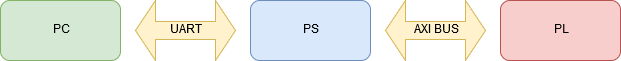
\includegraphics[width=0.65\textwidth]{figures/PCPSPL.png}
\caption{Draft of the test system}
\label{fig:draft}
\end{figure}

\section {Target Architecture}
The target architecture chosen is the Xilinx Zynq SoC. The idea of integrating processors, memories, mixed signal components with RF components in one chip has been known for a long time. Such Application Specific Integrated Circuits (ASICs) are designed to reduce size, to target more secure and faster communication between systems, to lower power consumption and increase reliability. The production cost of a single ASIC is also lower. The main problem of such full custom design is lack of flexibility, high, non-recurring development cost and time. Another important drawback is the lack of compatibility with most of standard applications which speed up the development process and, what comes with it, the time to market. Instead of full-custom ASICs, the semi custom SoCs with programmable logic are gaining on importance. Standard processors connected with Field Programmable Gate Arrays (FPGAs), peripherals and communication systems create an All-Pogrammable-System-on-Chip. The Programmable Logic is ideal for implementing high-speed logic and data flow systems, while Processing System supports operating system and standard software routines.The combination allows the developer to apply any system and easily partition it between hardware and software.

The Xilinx Zynq XC7Z020-1-CLG484 produced in 28nm technology is a SoC solution containing an ARM hardware processor with two cores and an FPGA in Artix-7 technology with 53200 LUTs, 106400 DFFs and 4.9 Mb of Block RAM. It supports all common standard communication interfaces: UART, SPI, CAN, I2C, GigE, GPIO and SDIO . It also allows quick data transfers between Pocessing System (PS) and Programmable Logic (PL) thanks to Xilinx AXI Bus. The full overview of the Zynq architecture is shown in \autoref{fig:Zynq}. The platform suits all needs of the hardware and middleware layer of the test bench.

\begin{figure}[H]
\centering
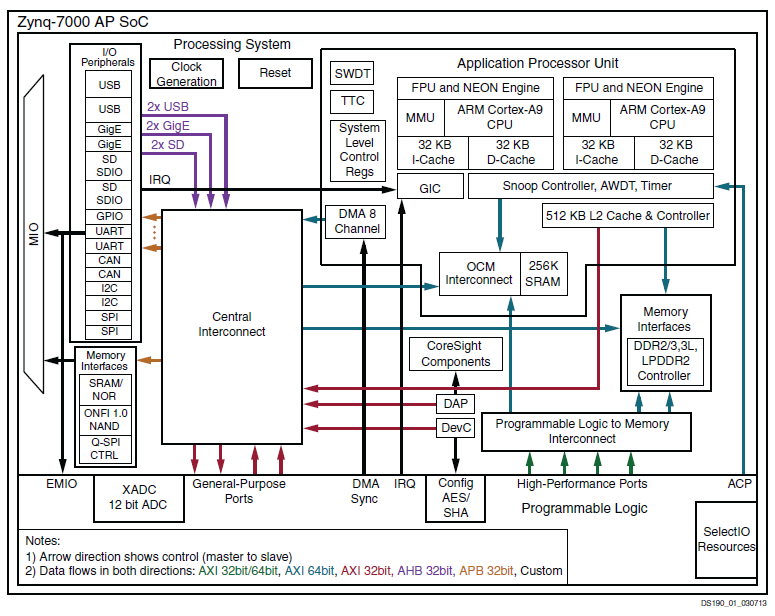
\includegraphics[width=0.65\textwidth]{figures/Zynq.png}
\caption{The Zynq Processing System~\cite{book:ZynqBook}}
\label{fig:Zynq}
\end{figure}

\subsection{FPGA Architecture}\label{ssec:SLICE}
Field Programmable Gate Arrays owe their name to the unique architecture of Configurable Logic Blocks (CLBs) connected with configurable interconnects and interfaced with configurable IOs. The configuration is stored as a program in the static memory and fed to the board as a serial bit stream. The CLBs in Xilinx 7-Series FPGA consist of two Slices, which are the smallest, repeatable structures. Each Slice includes four 6-input Look-Up-Tables (LUT), which can be configured to perform any logical operation on its inputs. Every 6-input LUT can be also used as two 5-input LUT, with common inputs but different functions, and therefore separate outputs. Every output can be stored in a flip-flop. Eight flip-flops, 4 LUTs, multiplexers and arithmetic carry logic form a Slice. Approximately two-thirds of all Slices are of SLICEL to implement logical operation and one-third - SLICEM for Block RAM and shift register implementation~\cite{report:CLB}.

\section{Middleware}
The middleware lays between the user application and the hardware. All of it's functionality is implemented within one core of the ARM processor available in Zynq. The middleware is implemented so that it has direct access only to the hardware modules via AXI interface. The modules are marked yellow in the \autoref{fig:testbench}. The program gathers the information received on UART and stores it in the fifo, from which it gets copied to the BRAM, until its full. Then it starts the test, by setting the ENA signal. The end of the test is indicated by the RDY signal. The program sends the content of the BRAM back to the PC application over UART. The user application can check the status of the middleware at any time, reading the frequency of the test, the status of all buffers and BRAMS.

\subsection{Communication protocol}
The communication protocol was implemented atop of the UART to control the test bench and feed it with data. The main idea behind the design, was its simplicity and the readability and not the performance. The protocol has evolved together with the application and the current version doesn't use all reserved bits. There is a lot of useless redundancy in the header, but the protocol is compliant with previous versions, which proved to be useful during the design. The PC application is the master and the middleware is the slave.

\begin{figure}[H]
\centering
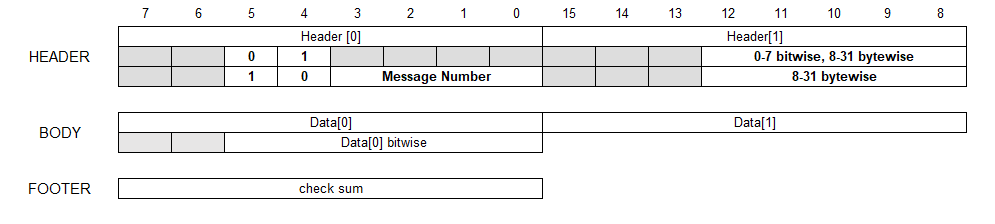
\includegraphics[width=\textwidth]{figures/SerialFrame.png}
\caption{Frame structure in the communication protocol}
\label{fig:Frame}
\end{figure}

The basic frame consists of a header, a body and a footer. The header is always 2 bytes long and it contains the information about the art of the following frame (bits 4:5) and its length (bits 8:12). There are two arts of frames, one to control the information flow, called the message frame and the other one to send the information. The protocol was constructed to support data transfers, that are not byte aligned, and thereby the length field has to be coded. Values $\leq 8$ denote the bit length and $8 <$ the length in bytes minus eight. The maximal frame size is 24 bytes ($2^5 - 8$). The footer is a check sum over all bytes of frame, it is one byte long. The information is always sent starting with the lowest byte. The frame structure is visible in~\autoref{fig:Frame}.

The communication starts with SYNC\_REQ awaiting the SYNC\_ACK. Every request is done by the master, who initiates the connection. After successful link creation, the master sends a STAT\_REQ signal to read all parameters from the test bench. The most important one is the BRAM capacity. The FREQ\_SET is sent to set the working frequency for the next test. To check the working frequency the FREQ\_GET is sent and the data is compared with the desired frequency. The response contains two values for two clocks in the test bench. The first clock is the UUT clock, the second one is the BRAM clock. If they lay within acceptance margin, the transmission of test vectors starts. Every 10th frame needs to be acknowledged by the slave with RECV\_ACK signal. If the signal doesn't arrive on time, the transfer is interrupted and the connection is reestablished. When the BRAM is full or all vectors have been sent, the master sends END\_OF\_F signal to terminate the transfer and indicate the start of the test. After the reception of END\_OF\_F the slave sets the ENA signal to start the hardware test procedure. The slave sends the results back without further request from the master side as soon as it receives the RDY flag from the hardware engine. The master checks if the received data is complete and starts the next transfer. There is a time limit for the test, which if exceeded resets the communication. The complete diagram of the communication is presented in the~\autoref{fig:UART}.

\begin{figure}[H]
\centering
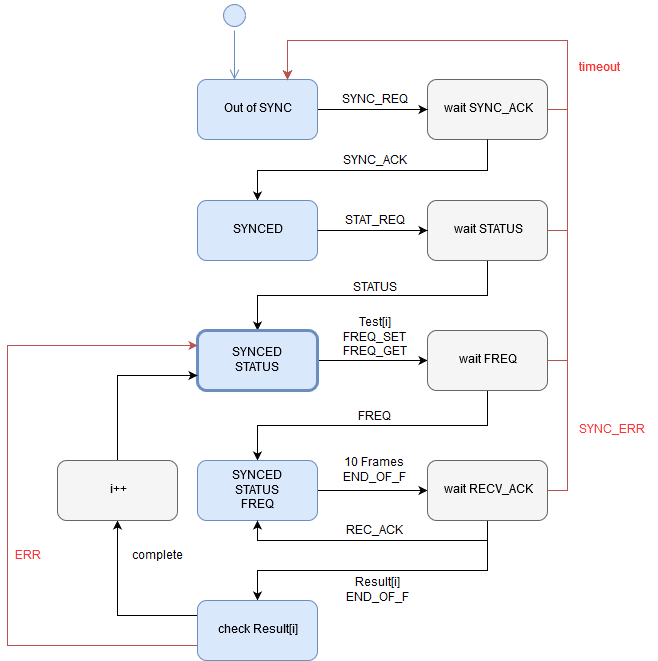
\includegraphics[width=0.65\textwidth]{figures/UART.png}
\caption{Diagram of master slave communication}
\label{fig:UART}
\end{figure}

\subsection{AXI Interface}
The communication between the PS and PL takes place entirely with use of AXI protocol. The PS writes and reads the BRAM contents, sets and gets the test frequencies and the ENA and RDY flags.\\
The history of the Advanced eXtensible Interface (AXI) goes back to year 2003 when it was first introduced as part of the ARM\textsuperscript{\textregistered} Advanced Microcontroller Bus Architecture (AMBA\textsuperscript{\textregistered}). The current version is called AXI4 and was released in 2010 as second version of AXI interface. The number four comes from the fourth version of AMBA, which contains AXI interface. The protocol is supported by many Intellectual Property (IP) producers (not only Xilinx) making the designer learn only one standard of communication. It was developed to standardize the communication between modules in the SoC designs. There are three types or modes of the AXI4:
\begin{itemize}
    \item AXI4 maps the memory of the interface and allows bursts up to 256 data transfers with just single address phase. Writing data to the memory, sends the data directly to the IP,
    \item AXI4-Lite is a light-weight version which offers just memory mapping without the burst capability,
    \item AXI4-Stream doesn't support any address phases. It allows unlimited burst of data. Lack of addresses makes it no more considered as a memory mapping interface.
\end{itemize}
The protocol works in the master slave system connecting both of them using an AXI Interconnect IP. It applies only to memory mapped versions, since the AXI4-Stream connects master and slave directly with each other or via DMA IP. The AXI Interconnect can service up to 16 masters and 16 slaves. Its main function is the data-width translation, downsizing too big master data packets into smaller slave-compliant bursts or upsizing it. It also does the clock-rate conversion, since both masters and slaves can operate on different clock frequencies. One of the big advantages of the interconnection is the mix support between protocol modes. Moreover the interconnection implements data pipelining for better frequency vs. latency trade-off. Finally it handles priorities in data transitions, making them either concurrent or using programmable priorities.
AXI4 protocol is designed for bidirectional communication, having separate write address, read address, write data, read data and write response channels in memory mapped modes and just data transfer channel in Stream mode. Every Xilinx IP has AXI4 support and there is an easy way of creating custom IPs supporting this protocol~\cite{report:AXI}.

\section{Physical Interface}
The physical interface of the test bench has to supply UUT inputs with test vectors and record responses of the outputs. It is advisable to incorporate the DfT techniques to increase controllability and observability of the UUT. But this step is not required to conduct tests, especially of relatively small modules. The system architecture is shown in \autoref{fig:testbench}.

\begin{figure}[H]
\centering
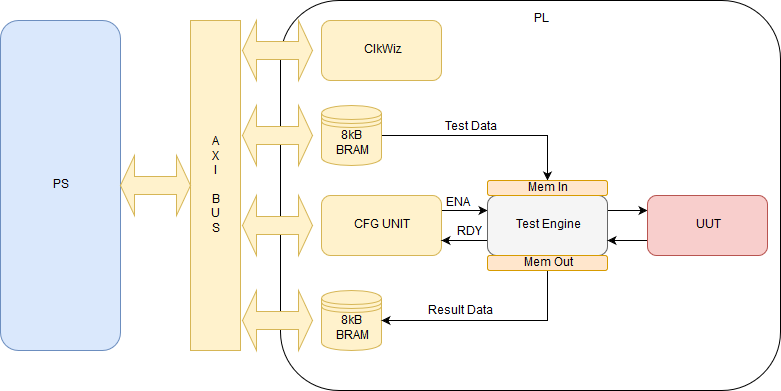
\includegraphics[width=0.65\textwidth]{figures/TestBench.png}
\caption{The Architecture of the test bench~\cite{book:ZynqBook}}
\label{fig:testbench}
\end{figure}


\subsection{Data Buffering}
There are two solutions that have been implemented and tested to deliver data to the inputs of the UUT
\begin{itemize}
    \item Direct mapping of the UUT as AXI IP. Every input of the UUT is mapped as different bit in the address space of the AXI interface. Clock input is also mapped in this fashion. The inputs are set to desired values, together with the low level of clock input. To achieve a rising edge of clock, the inputs are held constant for the time of the second transaction, but this time the clock bit is set to one. This scheme results in functional test of the design, without the ability to set the clock to any fix value. It's maximum frequency would be a half of AXI frequency and would amount in 100 MHz. To achieve this frequency, the middleware would have to schedule the bulk transactions of previously buffered data. This idea is showed in \autoref{fig:ver101}
\begin{figure}[h]
\centering
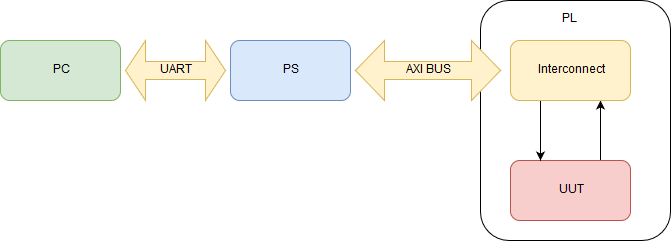
\includegraphics[width=0.65\textwidth]{figures/Version101.png}
\caption{Direct mapping of UUT over AXI interface}
\label{fig:ver101}
\end{figure}
    \item another solution is to buffer the data in the physical layer itself. Buffering limits the amount of data processed during one test run. After all data have been processed, the execution stops and doesn't restart until new data has been written to the memory. For the buffering, the internal Block RAMs have been used. Since they have dual port access, they fit perfectly for the scenario. The dual port capability of a memory implementation means concurrent access to the memory bank from two independent sources. They can be even clocked with two different clocks if necessary.~\cite{report:BRAM}.
    The BRAMs in the test bench are configured to be true dual ports. One port connected to AXI Bus and another port directly to the UUT. Conflicts must never occur because the memory is never accessed by PL and PS simultaneously. There are two instances of the BRAMs, one to supply the stimuli to the UUT, another to store responses. The input BRAM is filled with data. Then the ENA signal starts the test procedure, resulting in: valid responses stored in output BRAM and RDY signal, to indicate the end of the test procedure. The lack of simultaneous accesses from PL and PS would allow to use only one BRAM, connecting one port as the input to the UUT and another port as its output. After the end of test routine, it would be possible to switch the connection of one of the ports back to the AXI interface. This solution is more area efficient, but the presence of two BRAMS was determined by a possible extra feature of conducting successive runs with the same stimuli or chaining the output BRAM to be the input of another Test Engine. Hence the two BRAM solution is implemented.
    The drawback of this solution is the maximum frequency of the BRAM, which is 400 MHz. Additionally the clock has to be disabled whenever the data is replaced in the memory.
    \item To overcome the disadvantage of the previous solution, a fully customizable data buffering has been implemented. There are more than one vector stored in one memory word and they get fetched during one memory access. Then the vectors are shifted successively through the UUT. This buffering allows higher frequencies on the UUT side and lower on the memory side. The system was presented in the \autoref{fig:testbench}.
    The depth and width of the BRAMs may be adjusted to suit the testers needs and optimize BRAMs function. They have to be kept equal for both BRAMs at all times because the response vectors have the same length as the test vectors and there are exactly as many vectors stored in one memory word at the input and output. The width of the memory is a very important parameter for frequency multiplication. The $clk_{bram}$ is different then the $clk_{uut}$ and their relation $k$ is strongly connected with the width of BRAM word and the width of the UUT interface showed in~\autoref{eq:ratio}. 
    \begin{equation}
    k = \frac{clk_{uut}}{clk_{bram}} = \frac{width_{bram}}{width_{uut}}\label{eq:ratio}
    \end{equation}
    For example if the $width_{uut} = 8b$ and the desired test frequency set to $clk_{uut} = 300MHz$ and the BRAM configured to have $width_{bram} = 16b$ then it would have to be clocked with the frequency $clk_{bram} = 150MHz$ to satisfy data throughput. It usually makes sense to set the $width_{bram} > width_{uut}$ to access frequencies higher then $clk_{bram_{max}} = 400 MHz$. The detailed explanation of the origin of this relation can be found in \autoref{ssec:engine}.
\end{itemize}

\subsection{Test Engine}\label{ssec:engine}
The main core of the test bench is the Test Engine which feeds the test vectors to the UUT and gathers the response vectors. It consists of two parts:
\begin{itemize}
    \item memory interface module with memory address generator, which calculates successive addresses for words in the memory bank and stores them in the input register every $clk_{bram}$ cycle. The addresses get incremented by $inc = width_{bram}/8$ due to the byte-wise addressing scheme. The memory interface also handles the write back of the response every $clk_{bram}$ cycle from the output register. The number of pipeline stages for memory data read operation has to be taken into account. The number of pipeline stages determines the delay in clock cycles when the information, stored under the address given in the address register, actually gets to the input register of the Test Engine. The pipeline is used by Xilinx to increase the clock rate of their BRAM modules~\cite{report:BRAM}.
    \item data downsize converter which reads input register and conducts parallel to parallel conversion where the input dimension is the $b=width_{bram}$ and the output dimension is the $u=width_{uut}$. The conversion process takes $k$ $clk_{uut}$ cycles where $k$ is calculated as showed in~\autoref{eq:ratio}. The Test Engine (\autoref{fig:testing}) successively shifts the $u$ size test vectors through the design. With each $clk_{uut}$ cycle new data is placed on the input of UUT and new response vector gathered.
    \item the upsize converter recombines the $u$ size responses into $b$ size word with another parallel to parallel conversion. The conversion is done by the shift register with parallel output. The functionality of shift registers is described together with the downsize conversion in the \autoref{subsec:mux}. The test vector and response vector have always the same width $u$, although the number of UUT inputs and outputs may vary. It is necessary to connect the unused ports of the Test Engine to a known constant value.
\end{itemize}
\begin{figure}[h]
\centering
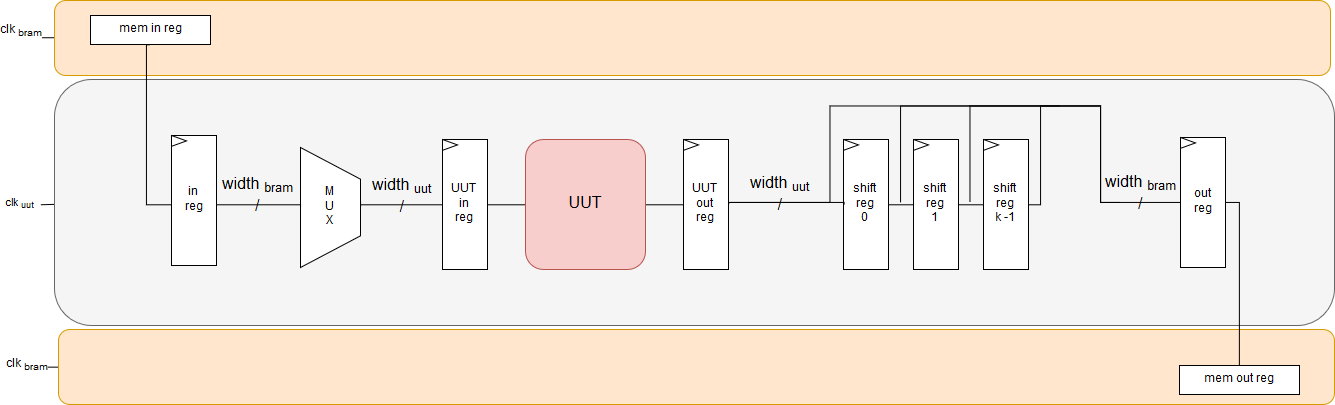
\includegraphics[width=0.65\textwidth]{figures/Test_Engine_complex.png}
\caption{Test engine architecture}
\label{fig:testing}
\end{figure}

The UUT is surrounded by flip-flops to guaranty, that the tested design is separated from the Test Engine logic. If it wasn't the case, the test procedure would include the test bench design and not only the UUT. Additionally the synthesis tool could combine some of the elements of the converters with the UUT logic. The structure of the Test Engine visible in \autoref{fig:testing} incorporates the idea of pipelining. Large functions are split into smaller atomic operations and the intermediate results are stored between the operations. This concept allows the whole logic to be clocked with higher frequencies, since the path from one register to the next one leads through only few logic gates or LUTs. 

When all buffered test vectores are processed and thereby all responses stored back, the Test Engine has to unplug the clock from the design. This procedure is conducted by special enable logic which switches on successive pipeline stages and switches them off together with the last valid input data.

\subsubsection{Data multiplexing}\label{subsec:mux}
Although the design is pipelined, the memory interface has it's limitations and cannot be possibly clocked with the working frequency of the UUT. To overcome this limitation, more than one test vector is stored in one memory word. After the word is fetched, the test vectors are successively shifted through the design. One of the ways to convert wide parallel inputs into series of narrower outputs can be accomplished using big multiplexer (MUX), or rather an array of MUXes. With each tact the converter chooses different part of the longer word to be routed to the output. The solution is shown in \autoref{fig:mux}. Number of MUXes in this solution is always equal to the number of outputs of the converter, with each MUX having as many inputs as the relation $k$. Therefore the solution can be achieved using $u$ $k$-to-1 MUXes.
\begin{figure}[h]
\centering
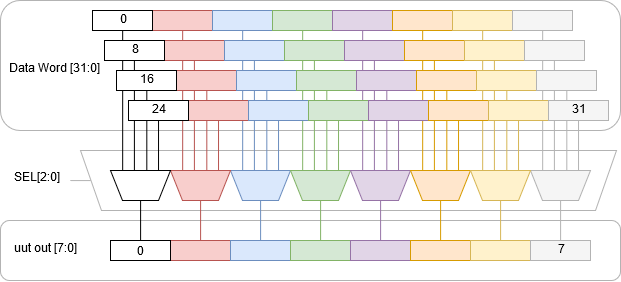
\includegraphics[width=0.65\textwidth]{figures/MUX.png}
\caption{32-to-8 bit converter using 8 4-to-1 MUXes}
\label{fig:mux}
\end{figure}

Another way of conducting a downsize conversion is by splitting it to many parallel to serial conversions. Such conversion can be achieved using shift registers with parallel input and serial output. Shift register consists of more chained registers, so that the output of the previous register is connected to the input of the next one. With each clock cycle the content of each register is copied to the following one. If the last register is connected to the first one, a circular shift is created. The difference between serial and parallel input shift register lays in the way of feeding it with data. In the serial shift register the input is connected to the first register and travels through all of the registers until it gets propagated to the last one. In the parallel input shift register all of the registers are written at once and shifted out one by one. The number of following registers is called the $depth$ of the shift register. With each cycle new vector occurs at the output until all vectors are processed. Then the shift register is loaded with all bits at once and the shifting starts over. The parallel input of shift register requires multiplexing to indicate whether the shift or write operation is going to happen. The shift registers can also have parallel output, meaning that all registers are read at once. The number of 2-to-1 MUXes needed for parallel input shift register is equal to, the depth of the shift register minus one, multiplied by its width. In the proposed solution there is a need of $(b-u)$ 2-to-1 MUXes and extra $k-1$ number of registers to create the shift register. The advantage of this solution are small MUXes with smaller delays, but the hardware overhead is significant. The shift register solution is shown in \autoref{fig:shift}.

\begin{figure}[h]
\centering
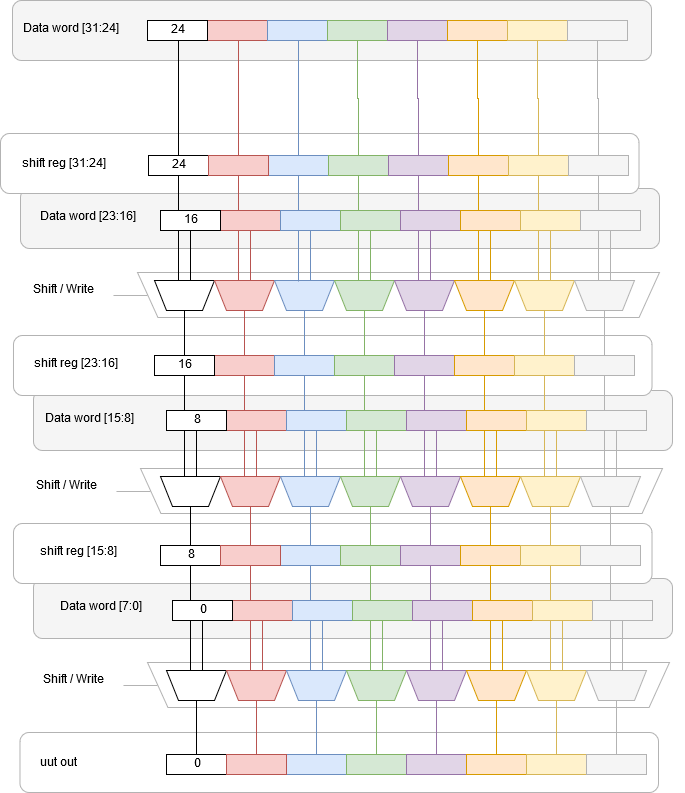
\includegraphics[width=0.65\textwidth]{figures/Shift_2.png}
\caption{32-to-8 bit converter using parallel input shift register and 24 2-to-1 MUXes}
\label{fig:shift}
\end{figure}

To provide the desired conversion each method involves different number of MUXes, therefore different complexity and delay. To compare both solutions, they need to be split into basic multiplexers. Assuming that every multi-input MUX can be broken into cascade of 2-to-1 MUXes, the comparison between the two methods is possible. The breaking method is shown in \autoref{fig:cascade}.

\begin{figure}[h]
\centering
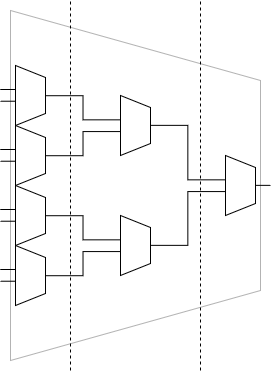
\includegraphics[width=0.25\textwidth]{figures/cascade.png}
\caption{Breaking of 8-to-1 MUX into several 2-to-1 MUXes}
\label{fig:cascade}
\end{figure}

Let's consider an $i$-to-1 MUX. Looking from the right-hand side of the \autoref{fig:cascade} the first cascade has always only one MUX. The next one has 2, and the next one 4. There are always twice as many MUXes in the next step as there were in the previous one. These values are terms of the geometric progression with common ratio $q=2$. The number of 2-to-1 MUXes needed to split an $i$-to-1 MUX into cascades is the sum $S_n$ of all $n$ terms of the progression starting with $a_1=1$ and ending with $a_n=\frac{i}{2}$. The \autoref{eq:nth} can be used to calculate the number of terms and the \autoref{eq:sum} the sum of the progression. After rearranging the terms in \autoref{eq:nth} for $n$ and substituting it with given values, the \autoref{eq:nthres} shows the number of terms in the progression and therefore the number of cascades of MUXes.
\begin{subequations}
\begin{align}
    a_n&=a_1\cdot q^{n-1}\label{eq:nth}\\
    \frac{a_n}{a_1} &=  q^{n-1}\\
    n &= \log_q \frac{a_n}{a_1}+1\\
    n &= \log_2 i\label{eq:nthres}
\end{align}
\end{subequations}
Using the \autoref{eq:sum} the sum of the progression and therefore the sum of all MUXes is calculated in \autoref{eq:sumres}.
\begin{subequations}
\begin{align}
    S_n&=a_1\cdot\frac{1-q^{n}}{1-q}\label{eq:sum}\\
    S_n&=\frac{1-2^{\log_2 i}}{1-2}\\
    S_n&=i-1\label{eq:sumres}
\end{align}
\end{subequations}

To compare both converting solutions, the one with multi-input MUXes has to be broken into cascades of 2-to-1 MUXes. There were $u$ $k$-to-1 MUXes needed in the first solution. Using the \autoref{eq:sumres} the number of 2-to-1 MUXes needed for this solution is $u(k-1)$. The second solution required $(b-u)$ MUXes, which can be calculated using \autoref{eq:ratio} as $(uk-u)=u(k-1)$. The number of 2-to-1 MUXes in both solutions is the same.

The hardware complexity doesn't have to necessary be mirrored in the implementation, because of different synthesis methods of multiplexing. The basic $k$-to-1 MUXes and shift registers were implemented and the number of required cells observed. The results are summarized in \autoref{tab:mux}.

\begin{table}[h]
\begin{tabular}{@{}lrrrrr@{}}
\toprule
Architecture & $k$-to-1 & LUT & FF & 2-to-1 MUX & lngst. path \\
\midrule
\multirow{6}{*}{MUX} & 2 & 1 & 0 & 0 & $LUT$ \\ 
                & 4 & 1 & 0 & 0 & $LUT$ \\ 
                & 8 & 2 & 0 & 1 & $LUT+MUX$ \\ 
                &16 & 4 & 0 & 3 & $LUT+2MUX$ \\ 
                &32 & 9 & 0 & 4 & $2LUT+MUX$ \\ 
                &64 & 17 & 0 & 12 & $2LUT+2MUX$ \\ 
\midrule
\multirow{6}{*}{Shift reg.}  & 2 & 1 & 1 & 0 & $LUT$ \\ 
                        & 4 & 3 & 3 & 0 & $LUT$ \\ 
                        & 8 & 7 & 7 & 0 & $LUT$ \\ 
                        &16 & 15 & 15 & 0 &  $LUT$ \\ 
                        &32 & 31 & 31 & 0 &  $LUT$ \\ 
                        &64 & 63 & 63 & 0 &  $LUT$ \\ 
\bottomrule
\end{tabular}
\centering
\caption{Utilization report for different $k$-to-1 converter architectures} \label{tab:mux}
\end{table}

The synthesis tool tries to split the logical operation, so that the implementation tool may maximally utilize the structure of CLBs and so that the performance is high, hence it implements the complex multiplexing as LUTs and MUXes. The speed of the conversion is constant in the shift register solution, because the signal has to travel only though one LUT at all times, but it also needs $k-1$ registers and LUTs. For bigger conversions this method is suggested. The big multiplexer method is better for smaller conversions, since the whole multiplexing may be fitted in one LUT or later in one SLICE for 8-to-1 conversion. Since $k$ was the number of test vectors in one memory word and therefore the ratio between clocks, the most common conversions will be up to $k/leq8$. There will be $u$ parallel conversions taking place and in worst case (8-to-1) the longest path will still stay within one SLICEL of the FPGA. This method is therefore present in the final version of the test bench.

\subsection{Configuration Unit}
To control the Test Engine, a configuration unit has been connected between the PS and PL. There are four registers that are accessible from the PS. Two registers when read, hold the actual frequency of both clocks, and the RDY flag, when written, they set the ENA flag, start and end address for BRAM operations and reset signal for the Test Engine and Frequency Monitors. The custom AXI IP is showed in the ~\autoref{fig:custom_ip}.

\begin{figure}[h]
\centering
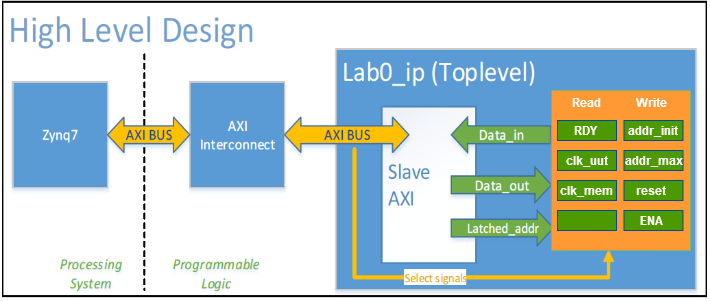
\includegraphics[width=0.65\textwidth]{figures/Custom_ip.png}
\caption{Configuration Unit AXI Custom IP based on~\cite{report:custom_ip}}
\label{fig:custom_ip}
\end{figure}

\subsection{Configurable Clock}
One of the crucial tasks of the test bench is the ability to test the design with different frequencies. The frequency has to be dynamically adjustable and stable at all times. The dynamical synthesis of the clock is possible thanks to Mixed-Mode-Clock-Manager (MMCM)~\cite{manual:MMCM}. The MMCM is shown in the~\autoref{fig:MMCM}. There are two input clocks and two reference clocks. Both input clocks are divided by coefficient D at their input. The input signal and reference signal enter the pulse frequency detector (PFD), which detects the phase shift and frequency difference between the input and reference clocks. It produces the up and down signals for charge pump (CP) and loop filter (LF) to influence their outputs. If the frequency is too high, the down signal indicates, that the CP should lower its output voltage, which manipulates the voltage controlled oscillator (VCO). If the frequency is too high, the down signal is sent. The VCO is connected with seven counters, that can have adjustable outputs. The eighth counter is a feedback counter for additional fractional divide (M) of the reference clock and therefore of the output clocks. When the output clock frequency is stable, on all outputs, a locked signal is set.

\begin{figure}[h]
\centering
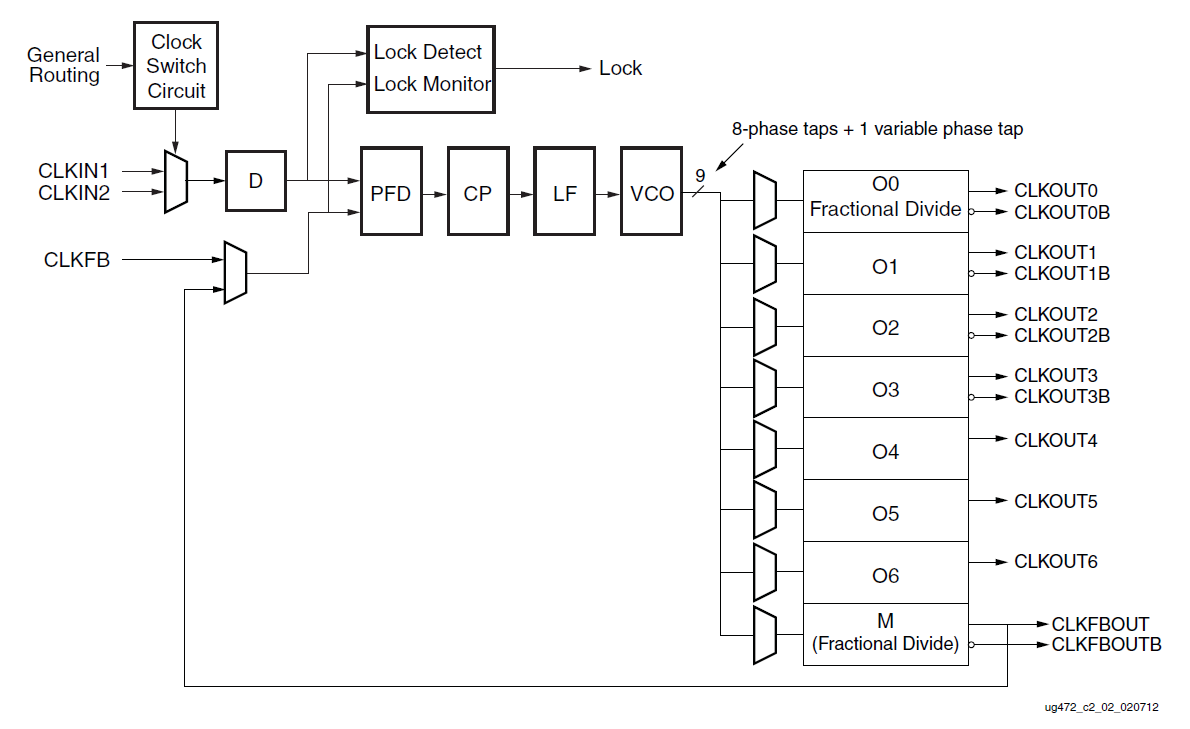
\includegraphics[width=0.65\textwidth]{figures/MMCM.png}
\caption{Deteiled MMCM Block Diagram~\cite{manual:MMCM}}
\label{fig:MMCM}
\end{figure}

In the current version of the test bench, only the prescaling of clocks is used. There is no phase shift required. The parameters D and M define the frequency of the VCO. The parameter O0 changes the $clk_{uut}$ frequency and the parameter $O1$ - the $clk_{BRAM}$. During the parameter change, the clock output is unstable, therefore the change happens between tests and not during the test. All parameters are adjustable via AXI interface. 

There are many valid parameter combinations, that result in the same output frequencies. According to~\cite{manual:MMCM} there is a following algorithm to be followed:
\begin{enumerate}
    \item constrain the M and D parameters to not generate the out of range frequencies 

    \begin{subequations}
        \begin{alignat}{4}
            & D_{MIN} &&=roundup(\frac{F_{IN}}{F_{PFD\_MAX}}),\quad && where \ F_{PFD\_MAX} && =450 \ MHz \label{eq:dmin}\\
            & D_{MAX} &&=rounddown(\frac{F_{IN}}{F_{PFD\_MIN}}),\quad  && where \ F_{PFD\_MIN} && =10 \ MHz \label{eq:dmax}\\
            & M_{MIN} &&=roundup(\frac{F_{VCO\_MIN}}{F_{IN}} \cdot D_{MIN}),\quad && where \ F_{VCO\_MIN} && =600 \ MHz \label{eq:mmin}\\
            & M_{MAX} &&=rounddown(\frac{F_{VCO\_MAX}}{F_{IN}} \cdot D_{MAX}),\quad && where \ F_{VCO\_MAX} && =1200 \ MHz \label{eq:mmax}
        \end{alignat}
    \end{subequations}
For $F_{IN} = 100 \ MHz$, which is a system clock provided as the input to the MMCM unit, parameters $D \in [1,10]$ and $M \in [6,120]$. The maximal output frequency is 800 MHz according to the Clock Wizard in Xilinx IP Integrator. It is possible to dynamically change the frequency to be higher then this limit.
    \item after specifying the input frequency, there are many possible parameter combinations that produce desired output frequency. The goal is to find such pair of $M$ and $D$, so that the $F_{VCO}$ is maximal, while the parameters are both minimal. There is a suggested formula to calculate an ideal M parameter first, starting with minimal D value.
    \begin{equation}
         M_{IDEAL} = \frac{D_{MIN} \cdot F_{VCO\_MAX}}{F_{IN}} \label{eq:mideal}
    \end{equation}
    According to \autoref{eq:mideal} the $ M_{IDEAL} = 12$ and therefore the $F_{VCO\_IDEAL}=F_{VCO\_MAX}=1200 \ MHz$. 
\end{enumerate}
Let's try to set the parameters for two output frequencies $F_{UUT} = 112 \ MHz$ and $F_{MEM} = 28 \ MHz$. The VCO frequency is common for all output clocks. Since both frequencies in the test bench are always related by the ratio, the $O$ parameters of output counters will always have the same relationship. In this example it's $k=4$.
The \autoref{tab:MMCM} shows all possible parameters that should produce the desired output frequencies.

\begin{table}[h]
\begin{tabular}{@{}rrrrr@{}}
\toprule
D & M & VCO & O0 & O1 \\
\midrule
1 & 7.0 & 700 & 6.25 & 25 \\ 
2 & 14.0 & 700 & 6.25 & 25 \\ 
3 & 21.0 & 700 & 6.25 & 25 \\ 
4 & 28.0 & 700 & 6.25 & 25 \\ 
5 & 35.0 & 700 & 6.25 & 25 \\  
6 & 42.0 & 700 & 6.25 & 25 \\ 
7 & 49.0 & 700 & 6.25 & 25 \\ 
8 & 56.0 & 700 & 6.25 & 25 \\ 
9 & 63.0 & 700 & 6.25 & 25 \\ 
5 & 42.0 & 840 & 7.50 & 30 \\ 
5 & 49.0 & 980 & 8.75 & 35 \\ 
5 & 56.0 & 1120 & 10.00 & 40 \\ 
\bottomrule
\end{tabular}
\centering
\caption{All possible MMCM parameters} \label{tab:MMCM}
\end{table}

There are several possible results, that satisfy the algorithms requirements, depending on which are more important. The minimal values of $M$ and $D$ are $D=1$ and $M=7.0$, the closest values to the ideal $M$ are $D=2$ and $M=14.0$, the highest, and most optimal, $F_{VCO}$ is achieved when $D=5$ and $M=56.0$. The Xilinx Customization Tool for Clock Wizard (v5.3) IP in Vivado 2016.3 sets the $M = 49.0$ and $D=5$, which gives $VCO = 980\ MHz$. Neither $M$ nor $D$ are minimal and they don't result in the maximal $VCO$. There is not enough information in the user guide to determine how exactly is Xilinx choosing the right parameter set.

To find the right parameters, all combinations have been generated and tested. Not all have been successfully synthesized in the design, although the parameters laid in the allowed range. There were more parameter combinations possible for each output clock rate and always the first lucky choice has been saved. There were some output clocks that were not reached. The PC application loads the parameters from the file at the start up and if the desired test frequency is not listed, the tool uses the closest one from the list. This approach saves a lot of time, which would be otherwise wasted on trying to guess the successful combination.
\subsection{Clock Monitor}
To check if the desired frequencies in the design are properly set, there are two clock monitors, that count clock pulses during specified time. The number of pulses is then processed in the middleware and passed to PC application as frequency value. 

One clock monitor contains two counters, one counts pulses of the variable clock and the other of the reference clock. There are two monitors, one per each clock in the test bench. The measurement time depends on the length of the reference counter. In this example it is 13 bits. Half for the measurement ($2^{12}$) and half for latching the data out and reseting the counter. This approach guaranties a proper clock domain crossing. The reference clock is a 100 MHz system clock, which gives a total measurement time of $10ns \cdot 4096 \approx 40 \mu s$. Every $80 \mu s$ a new value of the reference counter is visible on the output. The output is mapped thanks to AXI bus and can be read directly in the middleware. The variable counter is 16 bit long, so the variable frequency can be $2^{16}/2^{12} = 2^4 = 16$ times faster then the reference clock. It gives unreachable 1,6 GHz. The output signal can be latched during 1024 cycles of the reference clock, making the minimal frequency of the variable clock to be $100MHz\ / 1024 \approx 100 \ kHz$. The example of clock monitor wave diagram is shown in \autoref{fig:clk_monitor}. The reference counter is 4-bit long (3-bit for test) and the time window for signal output is just 2 clock cycles. Hence the test clock may not be more than 2 times slower then the reference clock. The output frequency is calculated as 
\begin{equation}
    \frac{cnt_{test}}{cnt_{ref\_max}/2}\cdot f_{in} = 4/8 \cdot 100 \ MHz = 50\ MHz
\end{equation}
The output value is barely latched in the time window. The same concerns the reset signal. This is the minimum detectable frequency. On the other hand, If the variable frequency would exceed the 1,6 GHz, the variable counter would overflow before the test ends.

\begin{figure}[h]
\centering
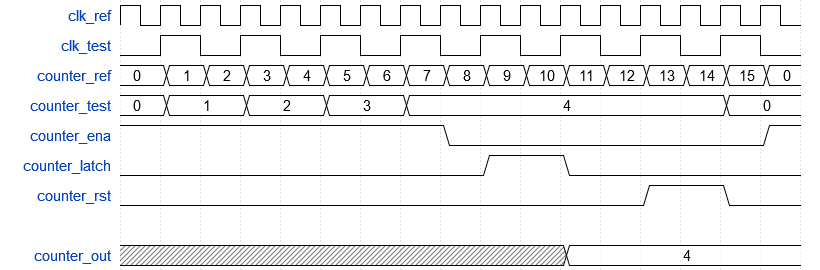
\includegraphics[width=\textwidth]{figures/clk_monitor.png}
\caption{Clock Monitor wave diagram}
\label{fig:clk_monitor}
\end{figure}

\section{PC Application}

The PC application communicates with the board over UART and is responsible for shifting the test patterns in and out. The test pattern generation and evaluation takes place in external software of test designers choice. All patterns used in this thesis were generated and evaluated using MATLAB 2015b. The application recognizes only specifically formatted XML entry file as test pattern. After the test is completed, the XML file is extended by UUT response. Additionally a HTML file is created to allow fast evaluation of the response. The application can accept more input files, processing them one after another. The general idea of the system functionality is presented in \autoref{fig:gui}.

\begin{figure}[h]
\centering
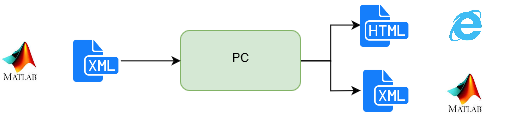
\includegraphics[width=0.65\textwidth]{figures/PC.png}
\caption{PC Application diagram}
\label{fig:gui}
\end{figure}

\subsection{Pattern Generation}
Test pattern generation occurs outside of the user application, which only processes the input XML file. The XML tree is shown in \autoref{fig:xml}. Every file may contain more then one configuration and every configuration - more then one test.

Every test has to consist of at least one, non-empty $DataInput$ element. Each character (either $0$ or $1$), stored as text, determines the state of the corresponding input during one clock cycle. Every input of an electronic circuit however has to be defined at all times, therefore not used inputs are all assigned to zero.

The monitoring of the output through $Expected$ element is not obligatory. The $Expected$ element serves for test evaluation purpose. If the user knows exactly what to expect on the output at any given time, the information will be compared by the application with the response of the test. If the comparison differs at any point, the test will be marked as faulty. The text in $Expected$ element consists of three characters: $0$, $1$ and $X$, where $X$ denotes ignored value. 
\\\\
Every text in every element within one test needs to have equal length!
\\\\
After the test is completed, the $ResultOut$ element is added to the output file for every $Expected$ element present in the input file. After the comparison, the attribute $passed$, with value $true$ or $false$, is added to the list of $Test$ element attributes. The HTML file also contains the indication of passed and failed tests, together with comparison results and positions of errors.

There are two important attributes in $AddConfiguration$ element. The $UUT\_width$ specifies the width of the UUT interface and how the data will be stored in the buffer. This attribute should be constant during all tests on one design, because it describes the physical state of the design and not the number of inputs used by the user during one test. The $Frequency$ attribute sets the desired test frequency. The PC application will choose the closest frequency from the list and run the test with this frequency. There is also a possibility to test the design for its maximum frequency or a range of different frequencies. To achieve that, the attribute $Frequency$ needs to be set to $0$. In this case the test engine will use the parameters configured in the GUI to perform the test.

\begin{figure}[h]
\centering
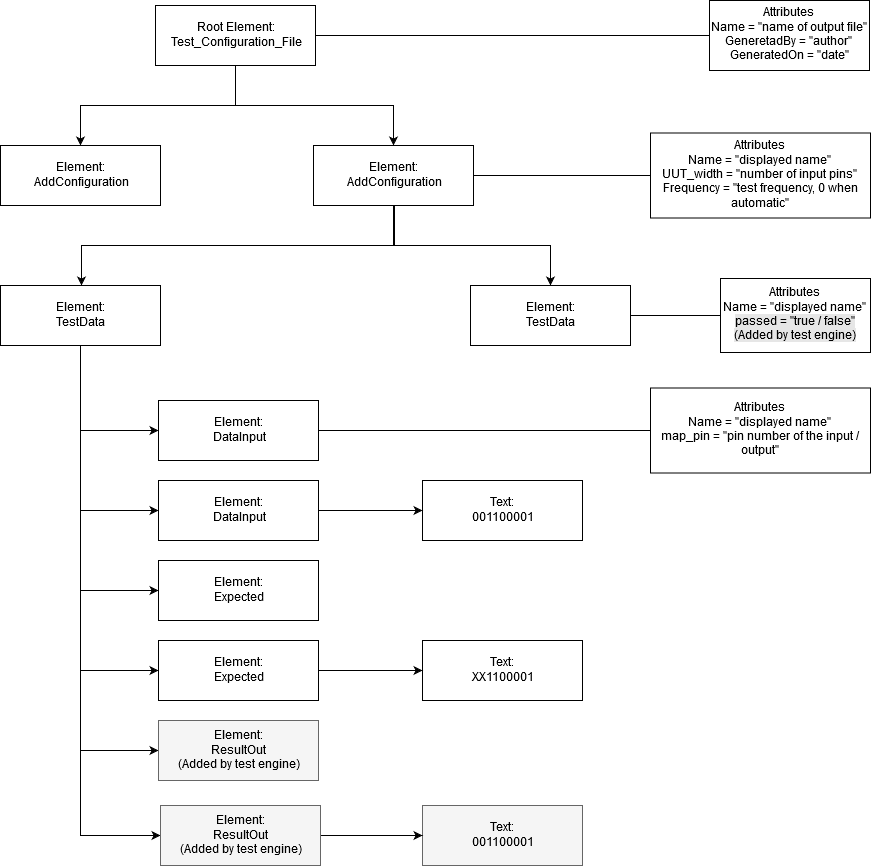
\includegraphics[width=0.8\textwidth]{figures/XML_tree.png}
\caption{Test Pattern XML tree}
\label{fig:xml}
\end{figure}

The parameters are: the start frequency, the initial step and the maximal frequency. The application will go through all frequencies between start and end with desired step, regardless of the test result. To test the design for its maximal frequency, the check-box $stop\_on\_fail$ needs to be checked. It will require some $Expected$ elements to be set in the test pattern, for the application to evaluate the response of the test and decide if test passed or failed. If the test fails, the frequency will be set back to the last successful one and the step will be lowered. The procedure repeats until the desired accuracy, adjustable by the minimal step parameter, is achieved.

\subsection{Data formatting}
The formatting of the data takes place already in the PC application and is stored in the memory unchanged. In the future the data could be sent compressed and formatted by the embedded processor, rather then prior to transmission, but in the current state it is done by PC, with utilization of parallel computing. The formatting depends on two factors: the width of a memory word and the width of the hardware interface. There are always more then one test vectors written to one memory word, because the $UUT\_width < MEM\_width$. Every bit in the test vector describes the state of one input during one clock cycle. The data is provided as separate streams for all inputs and need to be assembled into vectors and those need to be assembled into memory words. The process is shown in \autoref{fig:mem_word}. The processing is byte oriented, so the memory words are stored as byte array in the application memory. If the $UUT\_width<8$, then every byte consists of more vectors, if $UUT\_width>8$ - test vector consist of more bytes. The response data is received in the exact same format and needs to be disassembled using exactly the same principle.

\begin{figure}[h]
\centering
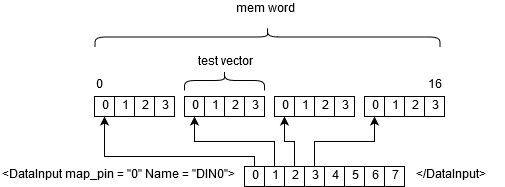
\includegraphics[width=0.65\textwidth]{figures/mem_word.png}
\caption{Memory Word assembly for $MEM\_widht = 16$ and $UUT\_width = 4$}
\label{fig:mem_word}
\end{figure}

\section{Limitations of the Test Bench}
To test the limits of the test bench and therefore be able to estimate the maximal working frequency for tests, a simple array of NOR gates have been used as UUT. Every signal is simply negated and returned. There will be exactly as many parallel LUTs as there are inputs to the UUT. If the LUT is not placed far away from the test bench, it is safe to assume, while testing single NOR function, that the longest path lays somewhere in the test bench. The following table shows the maximum frequency values achieved during the test.

\begin{table}[h]
\label{tab:max_freq}
\begin{tabular}{@{}llll@{}}
\toprule
UUT                       &mem\_width   &uut\_width &max. frequency \\ 
\midrule
\multirow{3}{*}{Inverter} &32           &4       & $\sim$536 MHz\\ 
                          & 32          & 8      & $\sim$500 MHz \\  
                          & 32          & 16     & $\sim$517 MHz \\ 
\bottomrule
\end{tabular}
\centering
\caption{Test for max. frequency}
\end{table}

After analyzing the results of the test of Inverter with 8 inputs, it started to generate errors at around 501 MHz. The simple comparison of expected values with response vectors didn't show any valuable information, except from many errors on all lines. This means, that the routing is not the problem, because that would result in just some lines failing and some preserving their functionality. After a closer look into the HTML file, a certain pattern is visible. The response seems to be shifted in relation to the expected signal. The analysis of XML file with MATLAB 2015b allows to calculate the shift with cross-correlation function. The result is shown in \autoref{fig:xcorr}. The received signal has to be shifted by 4 clock cycles to correspond to the expected signal. The shift amounts exactly the same number of clock cycles in all failed tests. Four clock cycles mean four test patterns that get lost at the beginning of the test. By this configuration, four test patterns create exactly one memory word, hence there is exactly one memory word missing, the first one. The address generator output is stored on negative memory clock edge, while the enable signal is generated on positive one. This is due to the fact, that the address and data has to be stable before the positive edge of memory clock. The circuit has therefore just a half of the clock cycle to calculate the first address, which leads to storing two words in the first location, hence the first word is overwritten, resulting in shift in response vector.

\begin{figure}[h]
\centering
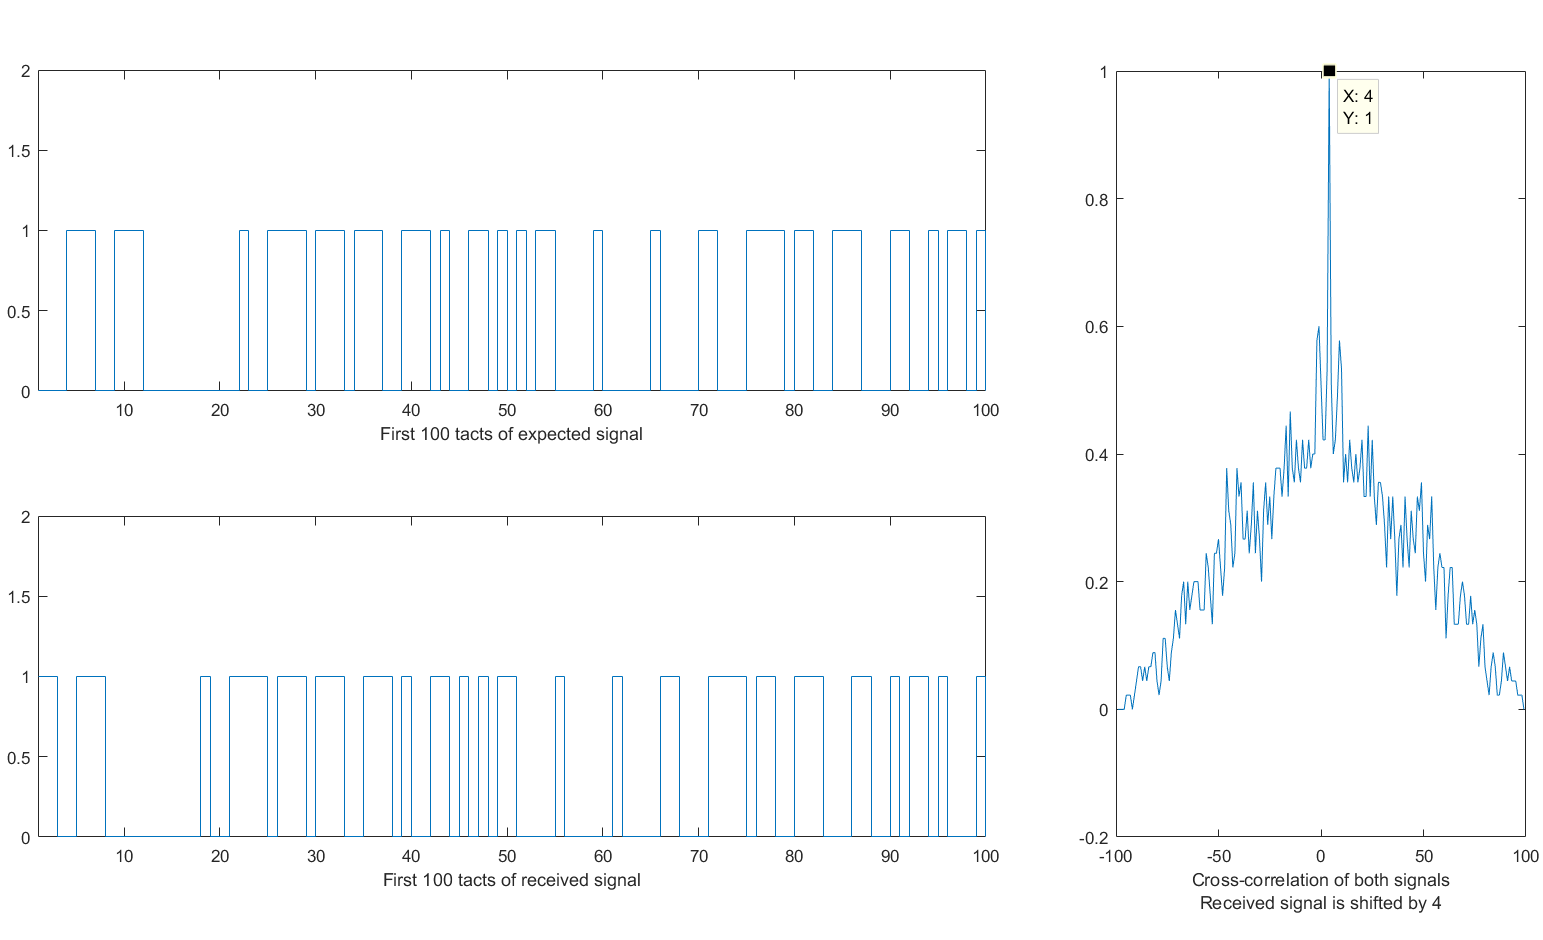
\includegraphics[width=\textwidth]{figures/Xcorr.png}
\caption{Cross-correlation of expected and received signals by 501 MHz}
\label{fig:xcorr}
\end{figure}

To achieve the highest frequencies, the tested designs have to be placed near the test engine or isolated with flip flops to prevent delay errors in interfacing signals, which could be misinterpreted as internal errors of the UUT.
